%%%%%%%%%%%%%%%%%%%%%%%%%%%%%%%%%%%%%%%%%%%%%%%%%%%%%%%%%%%%%%%%%%%%%%%%%%%%%%%%%%%%%%%%%%%%%%%%%
%
% Document:     Data Management  product tree
%
%%%%%%%%%%%%%%%%%%%%%%%%%%%%%%%%%%%%%%%%%%%%%%%%%%%%%%%%%%%%%%%%%%%%%%%%%%%%%%
\documentclass{article}
\usepackage{times,layouts}
\usepackage{tikz,hyperref,amsmath}
\usetikzlibrary{positioning,arrows,shapes,decorations.shapes,shapes.arrows}
\usetikzlibrary{backgrounds,calc}
\usepackage[paperwidth=78.0cm,paperheight=14.540000000000001cm,
left=-2mm,top=3mm,bottom=0mm,right=0mm,
noheadfoot,marginparwidth=0pt,includemp=false,
textwidth=30cm,textheight=50mm]{geometry}
\newcommand\showpage{%
\setlayoutscale{0.5}\setlabelfont{\tiny}\printheadingsfalse\printparametersfalse
\currentpage\pagedesign}
\hypersetup{pdftitle={DM products }, pdfsubject={Diagram illustrating the
                products in LSST DM }, pdfauthor={Autogenerated from MD}}
\tikzstyle{tbox}=[rectangle,text centered, text width=30mm]
\tikzstyle{wbbox}=[rectangle, rounded corners=3pt, draw=black, top color=blue!50!white,
                    bottom color=white, very thick, minimum height=12mm, inner sep=2pt,
                    text centered, text width=30mm]
\tikzstyle{pbox}=[rectangle, rounded corners=3pt, draw=black, top
 color=yellow!50!white, bottom color=white, very thick,
 minimum height=35pt, inner sep=2pt, text centered, text width=35mm]
\tikzstyle{pline}=[-, thick]
\begin{document}
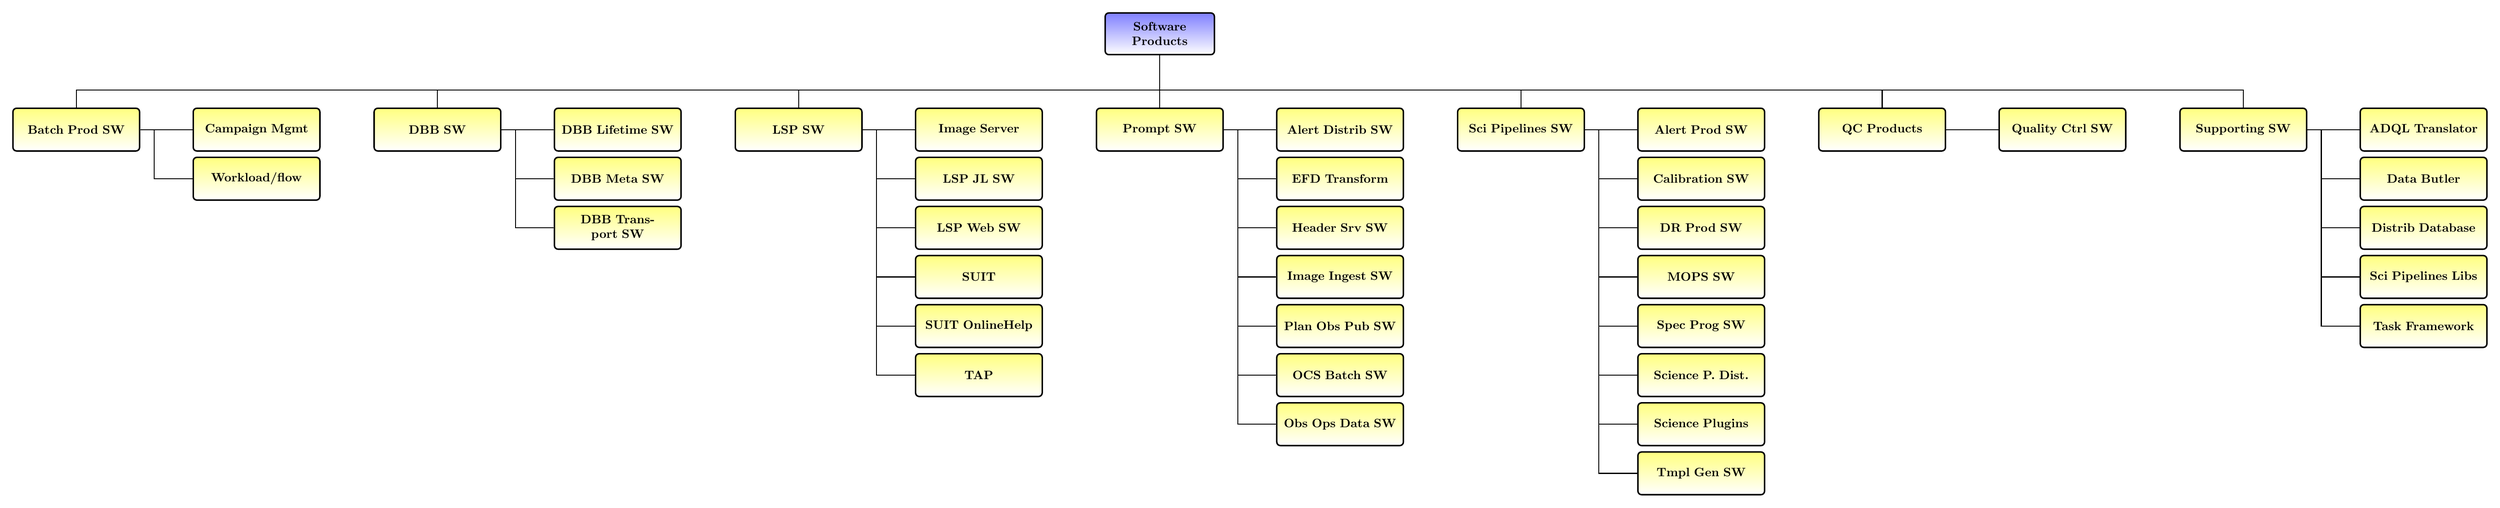
\begin{tikzpicture}[node distance=0mm]


\node (BPP) [pbox, 
] {\textbf{Batch Prod SW
} };
\node (CMPGN) [pbox,right=15mm of BPP] {\textbf{Campaign Mgmt
} };
 \draw[pline] (BPP.east) -| ++(0.4,0) |- (CMPGN.west); 
\node (WLWF) [pbox,below=4pt of CMPGN] {\textbf{Workload/flow
} };
 \draw[pline] (BPP.east) -| ++(0.4,0) |- (WLWF.west); 
\node (DBB) [pbox, 
right=6.7cm of BPP] {\textbf{DBB SW
} };
\node (DBBLIFE) [pbox,right=15mm of DBB] {\textbf{DBB Lifetime SW
} };
 \draw[pline] (DBB.east) -| ++(0.4,0) |- (DBBLIFE.west); 
\node (DBBMD) [pbox,below=4pt of DBBLIFE] {\textbf{DBB Meta SW
} };
 \draw[pline] (DBB.east) -| ++(0.4,0) |- (DBBMD.west); 
\node (DBBTR) [pbox,below=4pt of DBBMD] {\textbf{DBB Transport SW
} };
 \draw[pline] (DBB.east) -| ++(0.4,0) |- (DBBTR.west); 
\node (LSP) [pbox, 
right=6.7cm of DBB] {\textbf{LSP SW
} };
\node (DAXIMG) [pbox,right=15mm of LSP] {\textbf{Image Server
} };
 \draw[pline] (LSP.east) -| ++(0.4,0) |- (DAXIMG.west); 
\node (LSPJL) [pbox,below=4pt of DAXIMG] {\textbf{LSP JL SW
} };
 \draw[pline] (LSP.east) -| ++(0.4,0) |- (LSPJL.west); 
\node (LSPWEB) [pbox,below=4pt of LSPJL] {\textbf{LSP Web SW
} };
 \draw[pline] (LSP.east) -| ++(0.4,0) |- (LSPWEB.west); 
\node (SUIT) [pbox,below=4pt of LSPWEB] {\textbf{SUIT
} };
 \draw[pline] (LSP.east) -| ++(0.4,0) |- (SUIT.west); 
\node (SUITOH) [pbox,below=4pt of SUIT] {\textbf{SUIT OnlineHelp
} };
 \draw[pline] (LSP.east) -| ++(0.4,0) |- (SUITOH.west); 
\node (TAPSW) [pbox,below=4pt of SUITOH] {\textbf{TAP
} };
 \draw[pline] (LSP.east) -| ++(0.4,0) |- (TAPSW.west); 
\node (PR) [pbox, 
right=6.7cm of LSP] {\textbf{Prompt SW
} };
\node (ALRTDSTR) [pbox,right=15mm of PR] {\textbf{Alert Distrib SW
} };
 \draw[pline] (PR.east) -| ++(0.4,0) |- (ALRTDSTR.west); 
\node (EFDT) [pbox,below=4pt of ALRTDSTR] {\textbf{EFD Transform
} };
 \draw[pline] (PR.east) -| ++(0.4,0) |- (EFDT.west); 
\node (HEADER) [pbox,below=4pt of EFDT] {\textbf{Header Srv SW
} };
 \draw[pline] (PR.east) -| ++(0.4,0) |- (HEADER.west); 
\node (IIP) [pbox,below=4pt of HEADER] {\textbf{Image Ingest SW
} };
 \draw[pline] (PR.east) -| ++(0.4,0) |- (IIP.west); 
\node (OBSPUB) [pbox,below=4pt of IIP] {\textbf{Plan Obs Pub SW
} };
 \draw[pline] (PR.east) -| ++(0.4,0) |- (OBSPUB.west); 
\node (OCSBAT) [pbox,below=4pt of OBSPUB] {\textbf{OCS Batch SW
} };
 \draw[pline] (PR.east) -| ++(0.4,0) |- (OCSBAT.west); 
\node (OODS) [pbox,below=4pt of OCSBAT] {\textbf{Obs Ops Data SW
} };
 \draw[pline] (PR.east) -| ++(0.4,0) |- (OODS.west); 
\node (PRODN) [pbox, 
right=6.7cm of PR] {\textbf{Sci Pipelines SW
} };
\node (APPRMPT) [pbox,right=15mm of PRODN] {\textbf{Alert Prod SW
} };
 \draw[pline] (PRODN.east) -| ++(0.4,0) |- (APPRMPT.west); 
\node (DMCAL) [pbox,below=4pt of APPRMPT] {\textbf{Calibration SW
} };
 \draw[pline] (PRODN.east) -| ++(0.4,0) |- (DMCAL.west); 
\node (DRP) [pbox,below=4pt of DMCAL] {\textbf{DR Prod SW
} };
 \draw[pline] (PRODN.east) -| ++(0.4,0) |- (DRP.west); 
\node (MOPS) [pbox,below=4pt of DRP] {\textbf{MOPS SW
} };
 \draw[pline] (PRODN.east) -| ++(0.4,0) |- (MOPS.west); 
\node (SP) [pbox,below=4pt of MOPS] {\textbf{Spec Prog SW
} };
 \draw[pline] (PRODN.east) -| ++(0.4,0) |- (SP.west); 
\node (SPDIST) [pbox,below=4pt of SP] {\textbf{Science P. Dist.
} };
 \draw[pline] (PRODN.east) -| ++(0.4,0) |- (SPDIST.west); 
\node (SPLUG) [pbox,below=4pt of SPDIST] {\textbf{Science Plugins
} };
 \draw[pline] (PRODN.east) -| ++(0.4,0) |- (SPLUG.west); 
\node (TMPLGEN) [pbox,below=4pt of SPLUG] {\textbf{Tmpl Gen SW
} };
 \draw[pline] (PRODN.east) -| ++(0.4,0) |- (TMPLGEN.west); 
\node (QC) [pbox, 
right=6.7cm of PRODN] {\textbf{QC Products
} };
\node (QCSW) [pbox,right=15mm of QC] {\textbf{Quality Ctrl SW
} };
 \draw[pline] (QC.east) -| ++(0.4,0) |- (QCSW.west); 
\node (SUPPSW) [pbox, 
right=6.7cm of QC] {\textbf{Supporting SW
} };
\node (ADQL) [pbox,right=15mm of SUPPSW] {\textbf{ADQL Translator
} };
 \draw[pline] (SUPPSW.east) -| ++(0.4,0) |- (ADQL.west); 
\node (BUTLER) [pbox,below=4pt of ADQL] {\textbf{Data Butler
} };
 \draw[pline] (SUPPSW.east) -| ++(0.4,0) |- (BUTLER.west); 
\node (QSERV) [pbox,below=4pt of BUTLER] {\textbf{Distrib Database
} };
 \draw[pline] (SUPPSW.east) -| ++(0.4,0) |- (QSERV.west); 
\node (SCIPIPE) [pbox,below=4pt of QSERV] {\textbf{Sci Pipelines Libs
} };
 \draw[pline] (SUPPSW.east) -| ++(0.4,0) |- (SCIPIPE.west); 
\node (TXF) [pbox,below=4pt of SCIPIPE] {\textbf{Task Framework
} };
 \draw[pline] (SUPPSW.east) -| ++(0.4,0) |- (TXF.west); 
\node (DMSW) [wbbox, above=15mm of PR]{\textbf{Software Products
}};
 \draw[pline]   (BPP.north) -- ++(0.0,0.5) -| (DMSW.south) ; 
 \draw[pline]   (DBB.north) -- ++(0.0,0.5) -| (DMSW.south) ; 
 \draw[pline]   (LSP.north) -- ++(0.0,0.5) -| (DMSW.south) ; 
 \draw[pline]   (PR.north) -- ++(0.0,0.5) -| (DMSW.south) ; 
 \draw[pline]   (PRODN.north) -- ++(0.0,0.5) -| (DMSW.south) ; 
 \draw[pline]   (QC.north) -- ++(0.0,0.5) -| (DMSW.south) ; 
 \draw[pline]   (SUPPSW.north) -- ++(0.0,0.5) -| (DMSW.south) ; 

\end{tikzpicture}
\end{document}
